\title{Report of Conservation of Angular Momentum} % Title, modify to the name of experiment
\author{Haopeng Chen}% Author, modify to your name
\date{November 23rd, 2021}% Date, Modify to the DATE of EXPERIMENT


\documentclass[12pt]{article}
\usepackage{graphicx}
\usepackage{makecell}
\usepackage{float}
\newcommand{\diff}{\,\mathrm{d}}
\usepackage[margin=1in]{geometry}
\usepackage{fancyhdr}
\pagestyle{fancy}
\usepackage{extarrows}
\usepackage{breqn}
\usepackage[colorlinks,linkcolor=blue]{hyperref}
\newcommand{\N}{\mathbb{N}}
\newcommand{\Z}{\mathbb{Z}}
\newcommand{\trans}{^{\mathrm T}}
\usepackage[table]{xcolor}
\usepackage{bm}
\usepackage{array}
\usepackage[english]{babel}
\usepackage{natbib}
\usepackage{url}
\graphicspath{{images/}}
\usepackage{parskip}
\usepackage{fancyhdr}
\usepackage{vmargin}
\usepackage[font={bf, footnotesize}, textfont=md]{caption}
\usepackage{amsmath,amsthm,amssymb}
\usepackage{indentfirst}
\usepackage{bookmark}
\usepackage{fontspec}
\setmainfont{TeX Gyre Termes}
\setsansfont{TeX Gyre Heros}
\setmonofont{JetBrains Mono NL}
\usepackage{mathtools}
\usepackage{unicode-math}
\setmathrm{XITS Math}
\setmathsf{XITS Math}
\usepackage{listings}
\usepackage{ctex}

% 用来设置附录中代码的样式

\lstset{
    basicstyle          =   \ttfamily,
    keywordstyle        =   \ttfamily,
    commentstyle        =   \rmfamily\itshape,
    stringstyle         =   \ttfamily,
    % flexiblecolumns,
    numbers             =   left,
    showspaces          =   false,
    numberstyle         =   \ttfamily,
    showstringspaces    =   false,
    captionpos          =   t,
    frame               =   lrtb,
}

\lstdefinestyle{Python}{
    language        =   Python,
    basicstyle      =   \ttfamily,
    numberstyle     =   \ttfamily,
    keywordstyle    =   \color{blue},
    commentstyle    =   \color{green}\ttfamily,
    breaklines      =   true,
    % columns         =   fixed,
    basewidth       =   0.5em,
}





\newenvironment{theorem}[2][Theorem]{\begin{trivlist}
                \item[\hskip \labelsep {\bfseries #1}\hskip \labelsep {\bfseries #2.}]}{\end{trivlist}}
\newenvironment{lemma}[2][Lemma]{\begin{trivlist}
                \item[\hskip \labelsep {\bfseries #1}\hskip \labelsep {\bfseries #2.}]}{\end{trivlist}}
\newenvironment{exercise}[2][Exercise]{\begin{trivlist}
                \item[\hskip \labelsep {\bfseries #1}\hskip \labelsep {\bfseries #2.}]}{\end{trivlist}}
\newenvironment{reflection}[2][Reflection]{\begin{trivlist}
                \item[\hskip \labelsep {\bfseries #1}\hskip \labelsep {\bfseries #2.}]}{\end{trivlist}}
\newenvironment{proposition}[2][Proposition]{\begin{trivlist}
                \item[\hskip \labelsep {\bfseries #1}\hskip \labelsep {\bfseries #2.}]}{\end{trivlist}}
\newenvironment{corollary}[2][Corollary]{\begin{trivlist}
                \item[\hskip \labelsep {\bfseries #1}\hskip \labelsep {\bfseries #2.}]}{\end{trivlist}}
\DeclareMathOperator{\tr}{tr}
\DeclareMathOperator{\rank}{rank}
\DeclareMathOperator{\Span}{span}
\DeclareMathOperator{\row}{row}
\DeclareMathOperator{\col}{col}
\DeclareMathOperator{\range}{range}
\DeclarePairedDelimiterX{\inp}[2]{\langle}{\rangle}{#1, #2}
\DeclareMathOperator{\Proj}{Proj}
\DeclareMathOperator{\trace}{trace}
\newcommand{\Her}{^{\mathrm H}}
\DeclareMathOperator{\diag}{diag}
\makeatletter
\newcommand\fcaption{\def\@captype{table}\caption}
\makeatother
\setmarginsrb{3 cm}{2.5 cm}{3 cm}{2.5 cm}{1 cm}{1.5 cm}{1 cm}{1.5 cm}


\makeatletter
\let\thetitle\@title
\let\theauthor\@author
\let\thedate\@date
\makeatother

\pagestyle{fancy}
\fancyhf{}
\rhead{\theauthor}
\lhead{\thetitle}
\cfoot{\thepage}

\begin{document}
\rmfamily


\begin{titlepage}
  \centering
  \vspace*{0.5 cm}
  
\includegraphics[scale = 0.75,width=6cm]{CUHK}\\[1.0 cm]   % University Logo
  \textnormal{\large The Chinese University of Hong Kong, Shenzhen}\\[2.0 cm]
  \textnormal{\Large PHY 1002}\\[0.5 cm]
  \textnormal{\large Physics Laboratory}\\[0.5 cm]               % Course Name
  \rule{\linewidth}{0.2 mm} \\[0.4 cm]
  { \huge \bfseries \thetitle}\\
  \rule{\linewidth}{0.2 mm} \\[1.5 cm]

  \begin{minipage}{0.4\textwidth}
    \begin{flushleft} \large
      \emph{Author:}\\
      \theauthor
    \end{flushleft}
  \end{minipage}
  \begin{minipage}{0.4\textwidth}
    \begin{flushright} \large
      \emph{Student Number:} \\
      120090645  % Modify to your student number
    \end{flushright}
  \end{minipage}\\[2 cm]
  {\large \thedate}\\[2 cm]

  \vfill

\end{titlepage}

\tableofcontents
\pagebreak

\parindent=0.5in

% Introduction
\section{Introduction}
This experiment verifies the \emph{Conservation of Momentum} of a rotating disk by studying the \emph{Conservation of Angular Momentum}. In Newtonian mechanics, linear momentum, translational momentum, or simply momentum is the product of the mass and velocity of an object. It is a vector quantity possessing a magnitude and a direction. It is an important quantity in physics since it is a conserved quantity. That is, the total angular momentum of a closed system remains constant. During the motion of an object, the product of its velocity and its mass will not change. At the same time, the kinetic energy may be transformed into other forms of energy, presented as the loss of kinetic energy.\par
Hence, we conduct two experiments to verify the \emph{conservation of angular momentum}. A non-rotating ring was dropped onto a rotating disk in the first experiment. After a short collision, both the ring and the disk rotate at the same angular speed. This process was repeated three times to reduce the impact of random errors. In the second experiment, another disk was picked to replace the ring. This time, a non-rotating disk was dropped onto a rotating disk. Similarly, both of them rotate at the same speed after the collision. We conduct these two experiments upon a rotary motion sensor used to measure the disk's angular velocity with a diameter of about $9.5$cm, and an object that was dropped onto the disk. The relation between the initial rotational momentum and the final rotational momentum was explored in the experiment. Furthermore, in data analysis, all inertias and momentums of objects before and after the collision were listed in tables, and compared. We would also discuss estimated errors and the answers of experimental questions.

% Theory overview
\section{Theory}\label{sec:Theo}
Consider when a ring is dropped onto a rotating disk, there is no net torque on the system, since the torque on the ring is equal multitude and opposite in direction to one on the disk. Therefore, the angular momentum ($L$) is not changed and conserves.
\begin{equation}\label{eq:1}
  L=I_{\text{initial}}\omega_{\text{initial}}=I_{\text{final}}\omega_{\text{final}}
\end{equation}
where $I_{\text{initial}}$ is the initial rotational inertia and $\omega_{\text{initial}}$ is the initial angular speed. This assumes no torque is spawned inside the rotary motion sensor. This is not the fact, but the effect can be minimized by operating over as short a time as possible. We have also ignored the rotational inertia of the rotary motion sensor, which is quite small compared to that of the ring or the disk. The initial rotational inertia is that of a disk about an axis perpendicular to the disk and through the center of mass is
\begin{equation}\label{eq:2}
  I_{\text{initial}}=I_{\text{disk}}=\frac{1}{2}MR^2
\end{equation}
and the rotational inertia of the ring about an axis through its center of mass and parallel to the symmetric axis of the ring is
\begin{equation}\label{eq:3}
  I_{\text{rcm}}=\frac{1}{2}M(R_1^2+R_2^2)
\end{equation}
where $R_1$ and $R_2$ are the inner and outer radius of the ring. If the rotation axis is displaced by a distance $x$ from the center of mass, the rotational inertia can be calculated from the parallel axis theorem and we have
\begin{equation}\label{eq:4}
  I_{\text{ring}}=\frac{1}{2}M(R_1^2+R_2^2)+Mx^2
\end{equation}
Also, the rotational kinetic energy of a rotating object is given by
\begin{equation}\label{eq:5}
  E_{\text{k}}=\frac{1}{2}I\omega^2
\end{equation}

% Illustrate the Experiment Procedure
\section{Experiment Process}
\subsection{Setup}
At first, we fasten the \emph{rotary motion sensor} to the support rod and link it to \textit{PASCO 550 Universal Interface}. The support rod was tugged into the metallic base. After removing the small bolt fixed the transparent plastic pulley on the rotary motion sensor, we can take off the pulley and measure its mass and diameter. Although the pulley is not a standard disk, it can be consider as three concentric disks. Therefore, we can regard it as a uniform disk with the center of mass located at the center, and calculate is rotational inertia as a uniform disk with error small enough to ignore. After that, we use a digital balance to determine the mass of the rings, and use a caliper to measure their diameters. Finally, we use another same type of disk to conduct the second experiment. All data above are collected and shown in \hyperref[sec:raw]{Raw Data}.\par
\begin{figure}[H]
  \centering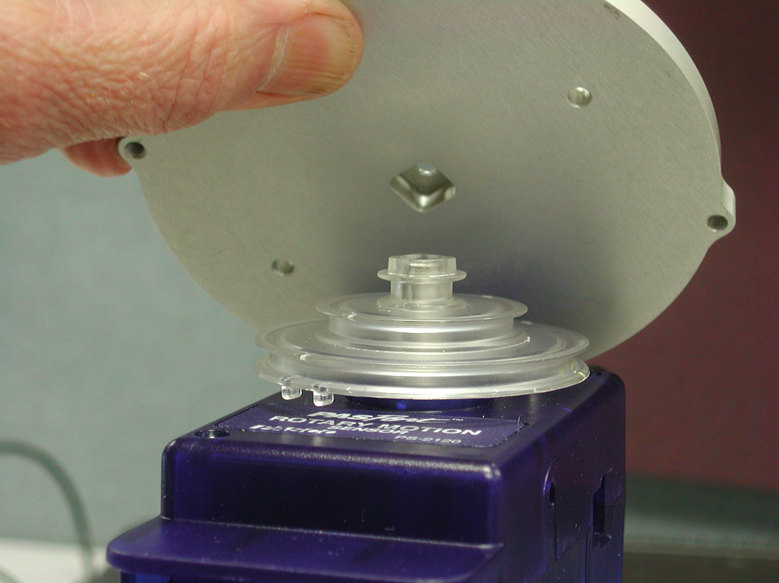
\includegraphics[width=15cm]{figSetup1.png}
  \caption{Attaching the Disk}
  \label{fig:attachDisk}
\end{figure}
After the basic measurement, we can put the accessories back. To avoid sliding during the rotation, the raised square of the pulley should be upward where corresponds to the area of the disk, as shown in Figure \ref{fig:attachDisk}.\par
Then, we put a level on the disk to check if the equipment is horizontal, which is crucial to get a good result. Once everything is ready, we finish this part done.
\begin{figure}[H]
  \centering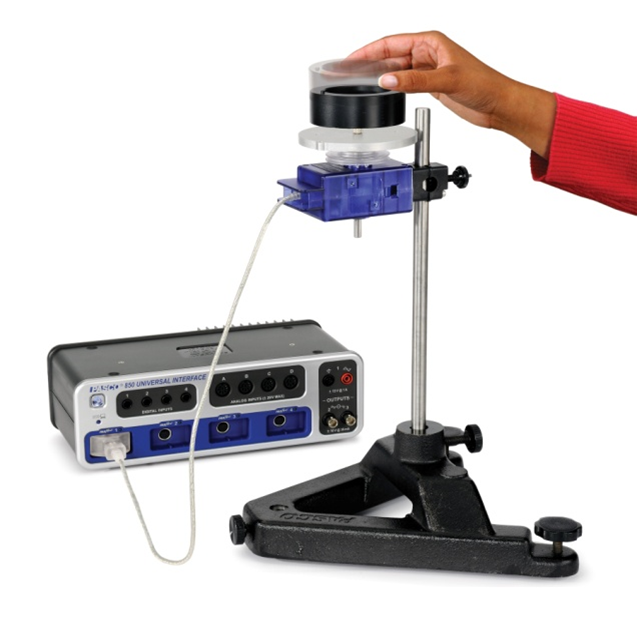
\includegraphics[width=15cm]{figSetup2.png}
  \caption{Setup}
  \label{fig:Setup}
\end{figure}

\subsection{Procedure A: Level Check}
To obtain expected result, it is significant to level the equipment before performing the experiment. We placed the ring onto the disk where its edge was tangent to the edge of the disk as shown in Figure \ref{fig:LevelCheck}.\par
\begin{figure}[H]
  \centering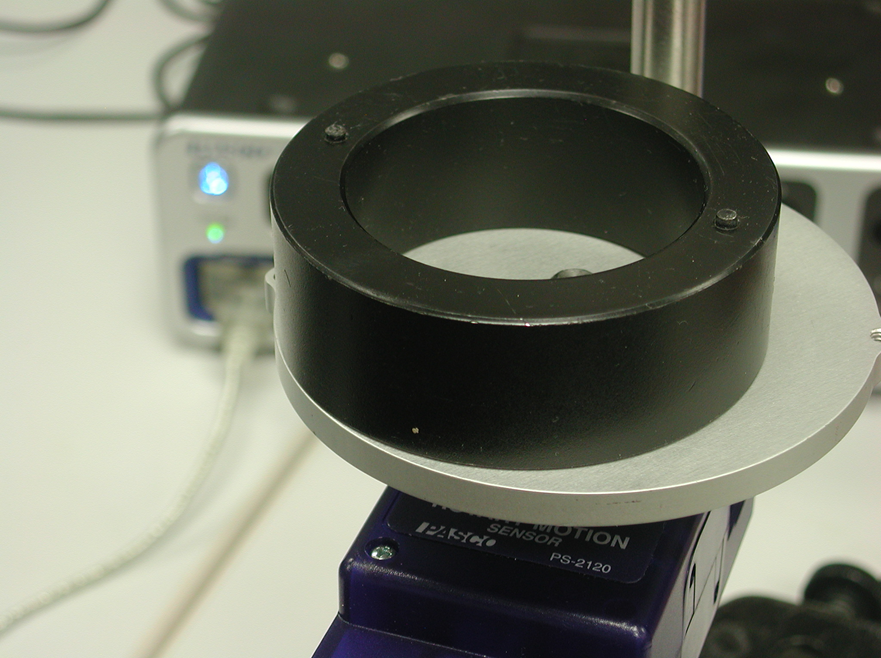
\includegraphics[width=15cm]{figLevelCheck.png}
  \caption{Offset Ring}
  \label{fig:LevelCheck}
\end{figure}
We use the rotary motion sensor to record the angular speed after a push is given to the disk. The disk with the ring should spin uniformly during the process of the motion. The curve of angular velocity would by a roughly a smooth linear one without periodic bumps caused by the ring when the ring speeds up going downhill and slows down going uphill during the rotation. We can modify the two adjustable feet of the stand bas to assure the bubble of the level always located at center, such a curve is placed as Figure \ref{fig:LevelCheck2}.
\begin{figure}[H]
  \centering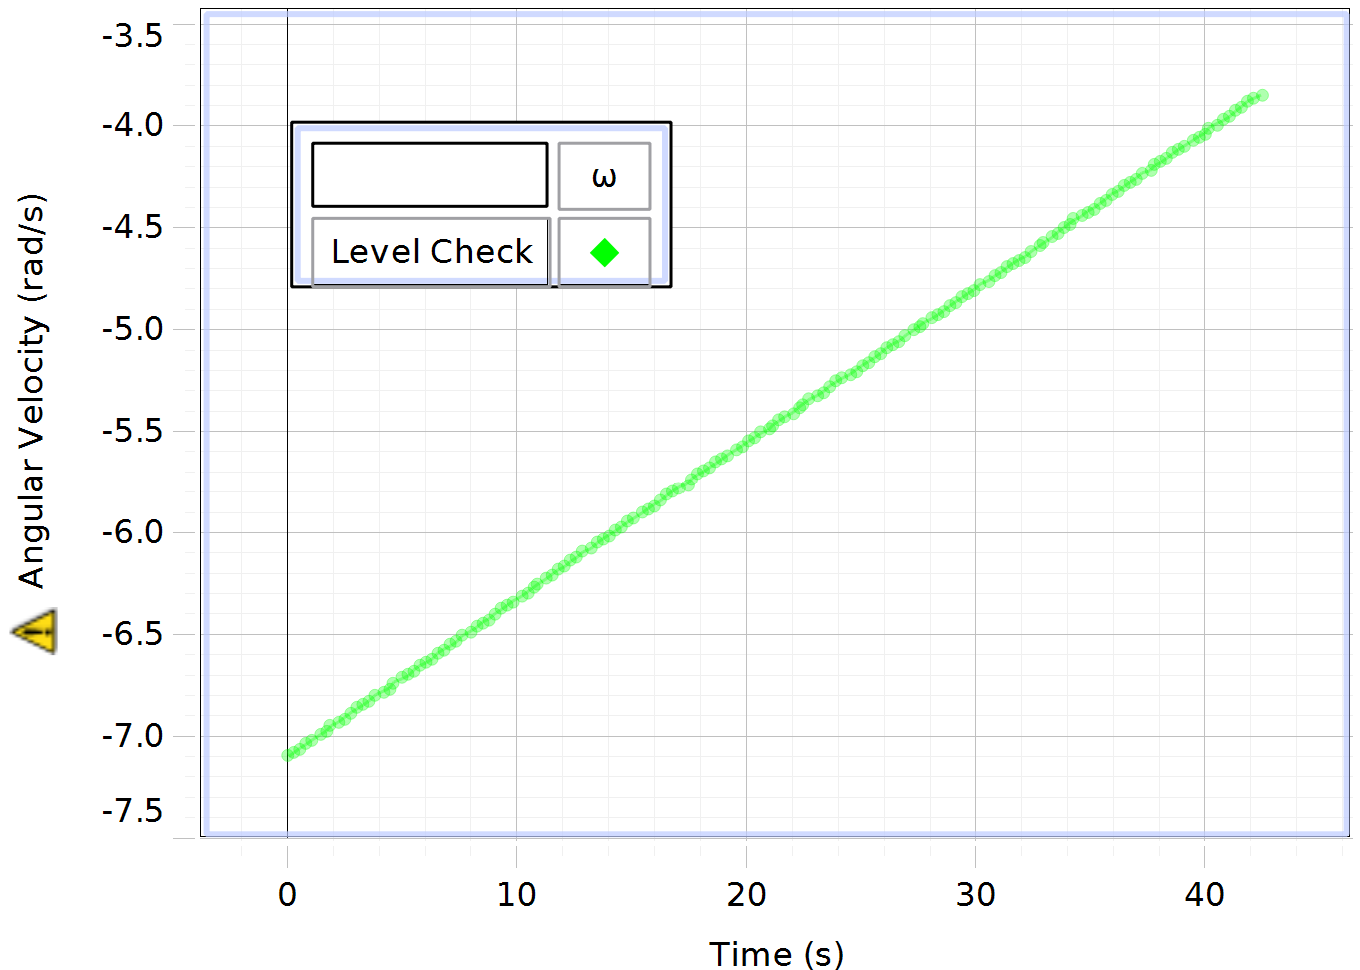
\includegraphics[width=15cm]{figLevelCheck2.png}
  \caption{Level Check}
  \label{fig:LevelCheck2}
\end{figure}

\subsection{Procedure B: Main Experiment}
First, the ring was held above the disk about $2$ to $3$mm to have a better result. Dropping the ring from too high would cause a relatively large force on the bearing resulting in a decrease of the angular momentum due to the friction. Likewise, getting fingers clear away from the ring in time was equally important.\par
The interface started to collect data after the disk was given a clockwise spin about $2$0 to $30$rad per second. Another two seconds later, the ring was released onto the spinning disk. The minimal distance from the edge of the ring to the edge of the disk was marked by an pencil and measured later. Then, we could calculate $x$ by:
\begin{equation}\label{eq:x}
  x=0.95\text{cm}-(\text{minimum distance})
\end{equation}
The same procedure was repeated two more times so that the result coming from the experiment would be more generalized.\par
Then, disk 2 replaced the ring. The square hold of the disk should be down-ward so that the bolt sticking up which fixes the lower disk would not collide the dropping disk.\par
After all runs have been done, four graphs of \emph{Angular Velocity versus Time} are made. By checking the curves, we get all the data needed in the analysis.



% Experiment Raw Data
\section{Raw Data}\label{sec:raw}
During the experiment, all \emph{Angular Velocity vs. Time} figures are generated by PASCO Capstone\texttrademark. Two special points have been set to each graph, the last one before collision and the first one after collision. So the velocities could be seen easily from the following figures:
\begin{figure}[H]
  \centering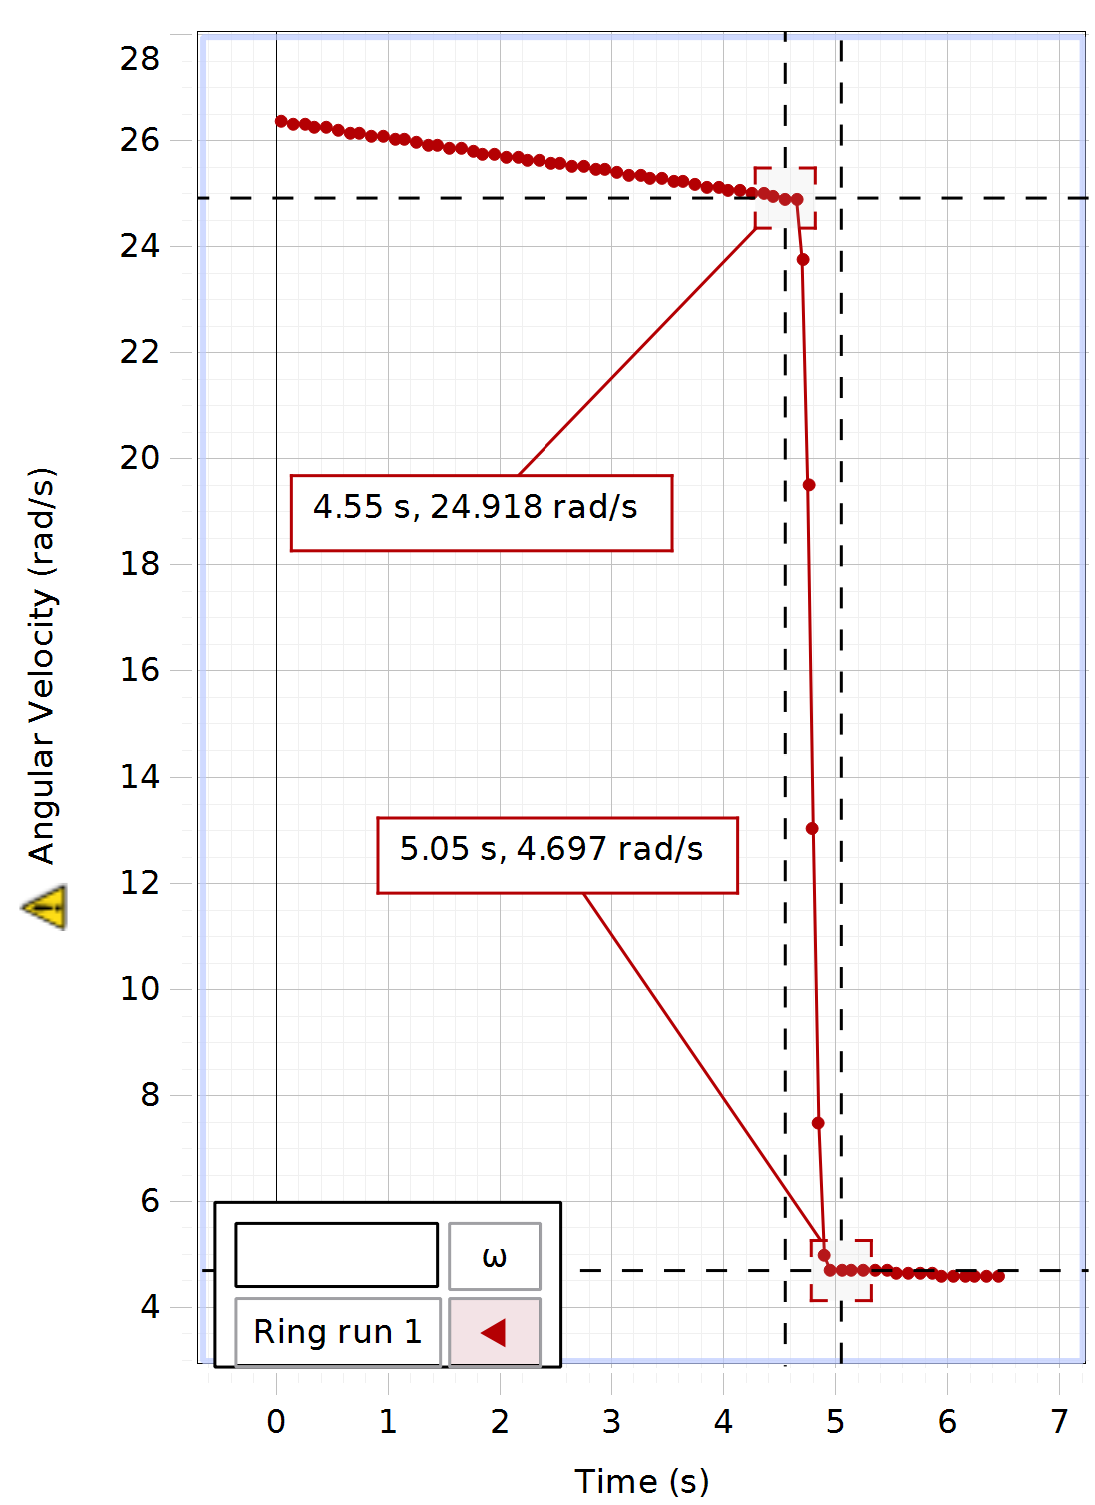
\includegraphics[width=15cm]{figRingRun1.png}
  \caption{Angular Velocity Change of Ring Run 1}
  \label{fig:RingRun1}
\end{figure}
\begin{figure}[H]
  \centering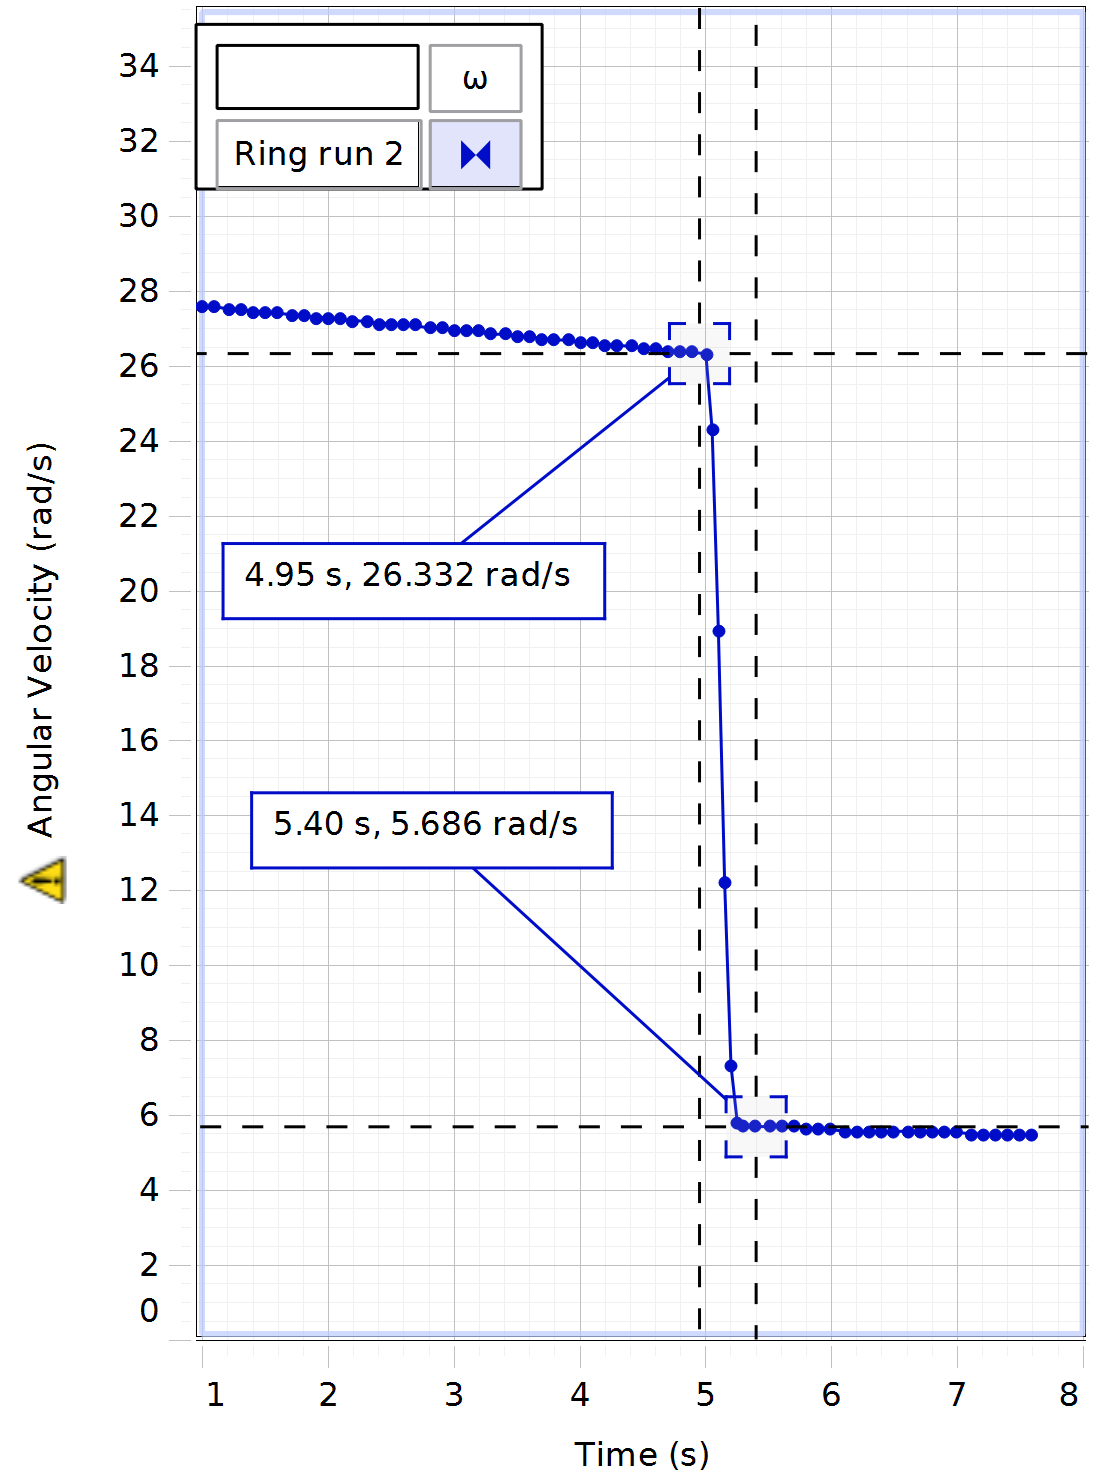
\includegraphics[width=15cm]{figRingRun2.png}
  \caption{Angular Velocity Change of Ring Run 2}
  \label{fig:RingRun2}
\end{figure}\begin{figure}[H]
  \centering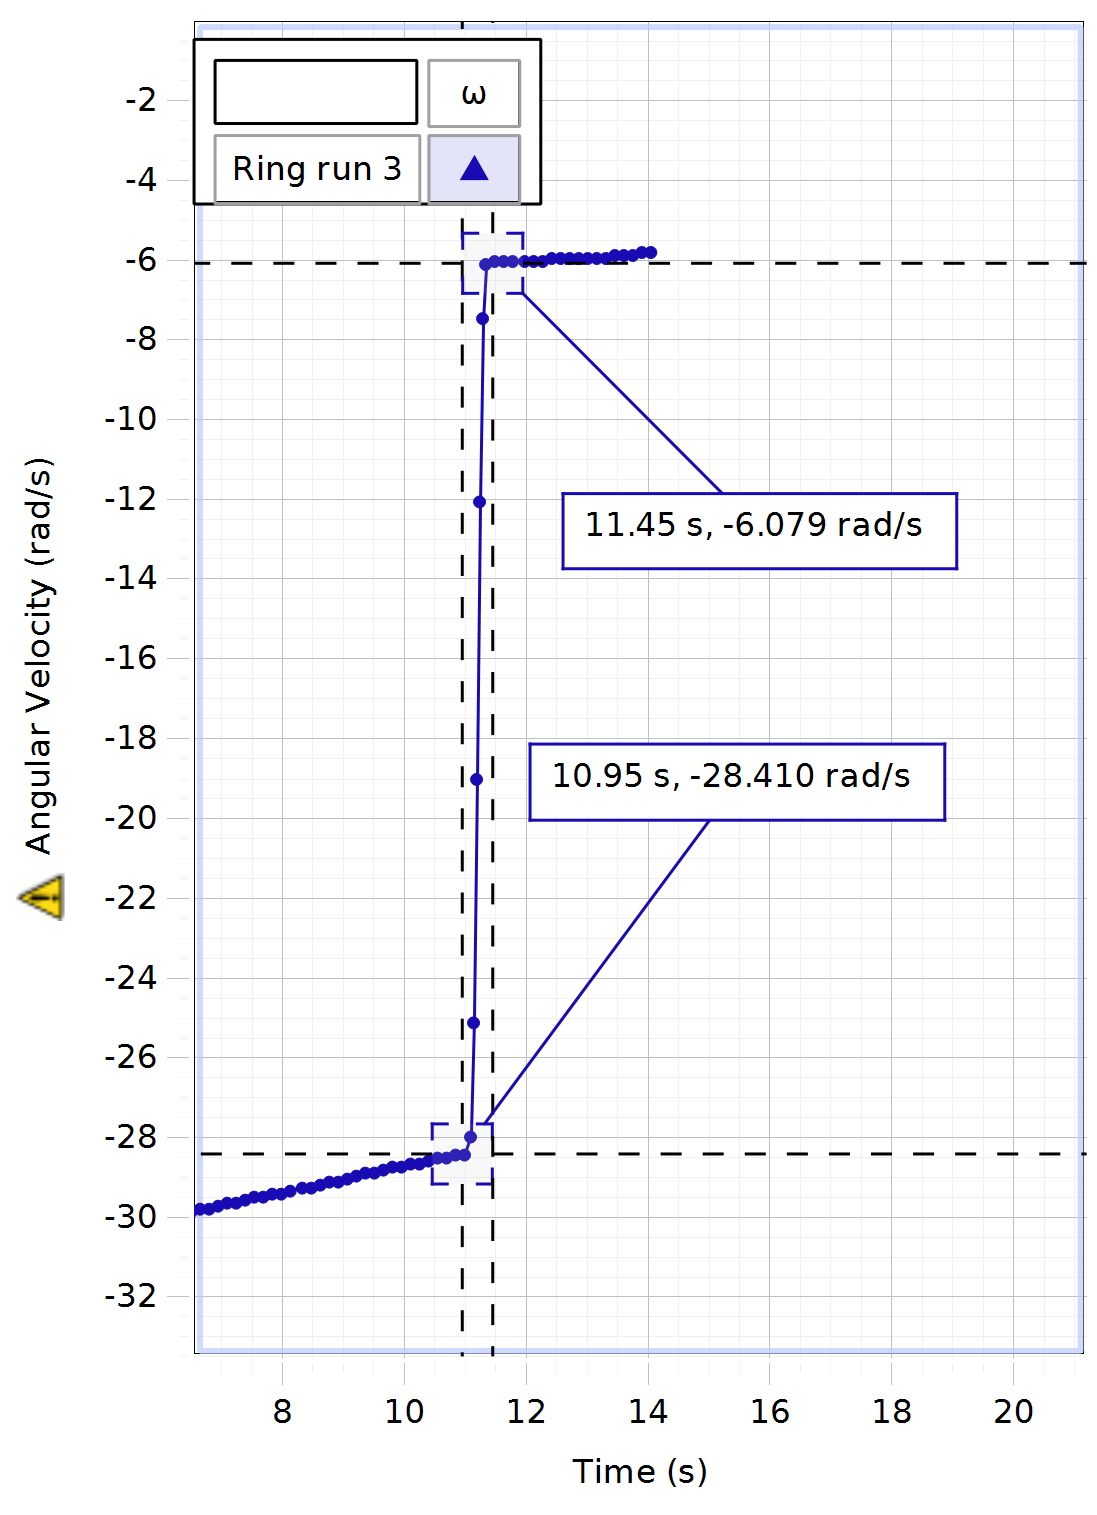
\includegraphics[width=15cm]{figRingRun3.png}
  \caption{Angular Velocity Change of Ring Run 3}
  \label{fig:RingRun3}
\end{figure}
\begin{figure}[H]
  \centering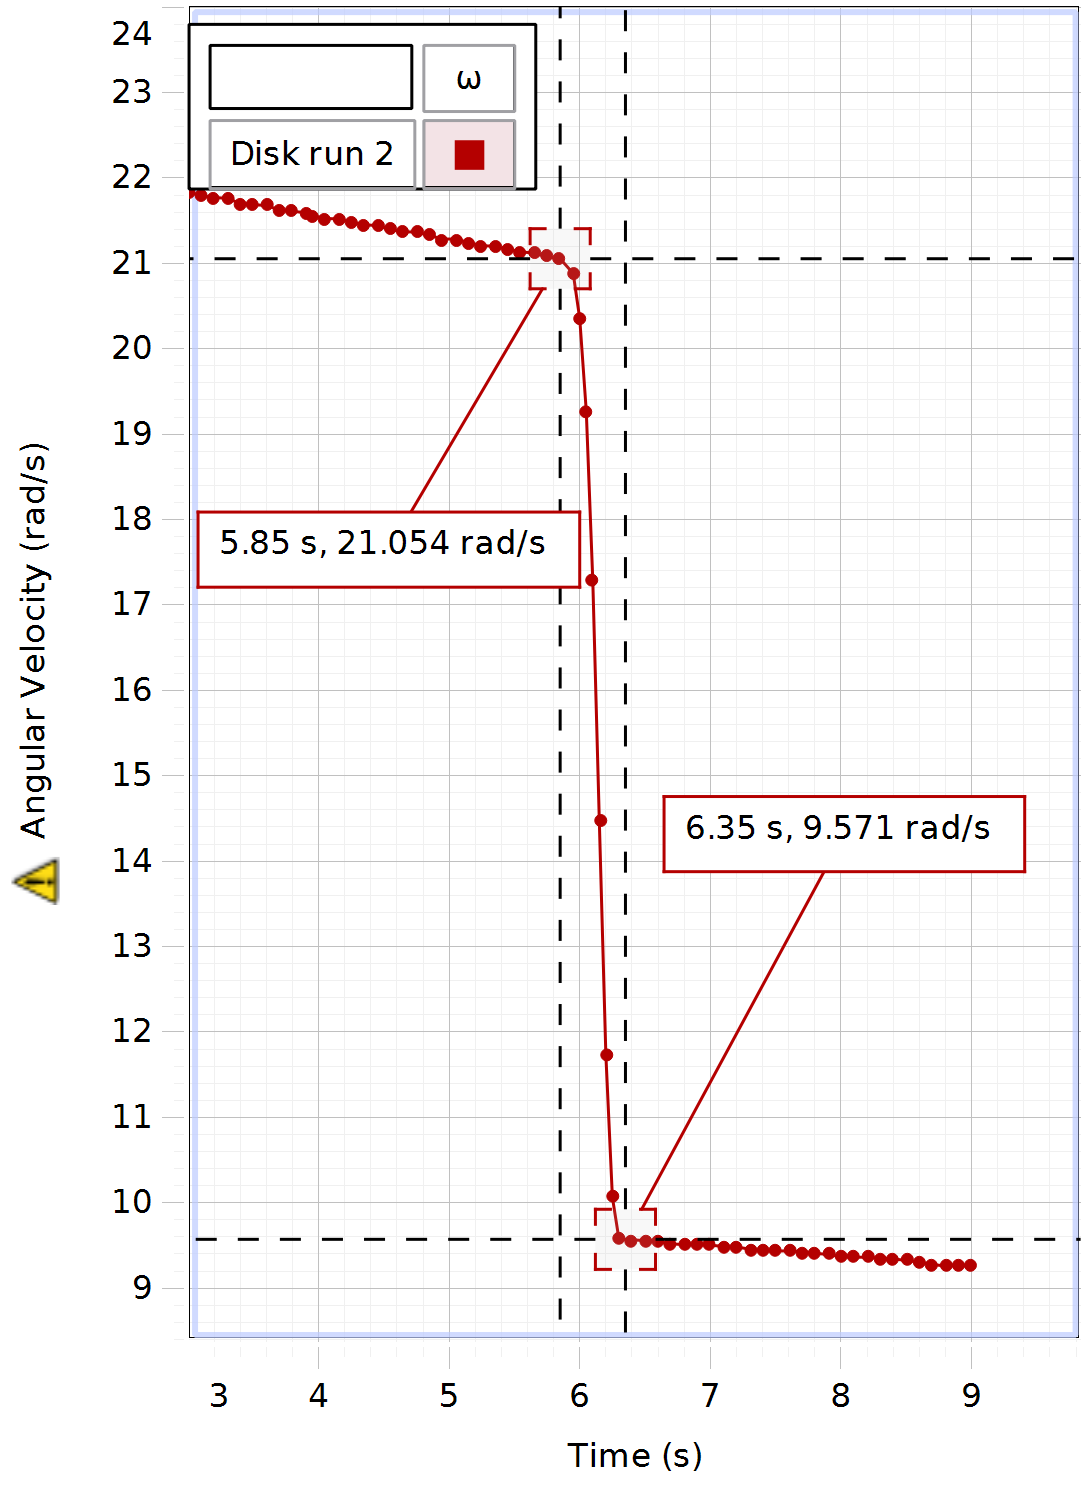
\includegraphics[width=15cm]{figDiskRun2.png}
  \caption{Angular Velocity Change of Disk 2 Run}
  \label{fig:DiskRun}
\end{figure}


\section{Analysis \& Questions}
\subsection{Analysis}
\paragraph{Mass}
We use a digital balance to determine the mass of objects in this experiment. Its expected estimated error is $\pm0.01$g.
\paragraph{Diameter}
We use a caliper to measure the diameter of the disks and rings. The resolution of the measurement is based on the minimal width of the sub-interval, which is $0.05$mm. Thus, the expected error would be $\pm0.005$cm.
\paragraph{Distance}
A ruler is used to determine the distance from the edge of the ring to the edge of the disk. As its resolution is $0.1$cm, the estimated error would be $\pm0.05$cm.
\paragraph{Angular Velocity}
During the experiment, a rotary motion sensor is used to detect the angular velocity of the rotating system. According to the official manual, the resolution of the sensor is $0.00157$rad, so we consider the estimated error as $\pm0.002$rad.\par
In the calculation procedure, the standard error of calculated data could be given by such a theorem.
\paragraph{Theorem}
If a function $k$ is determined by $n$ independent random variables, namely $p_1, p_2, ..., p_n\sim N(\mu, \sigma^2)$; that is, $k=f(p_1, p_2, ..., p_n)$. In this case, the standard error for $k$ is
\begin{equation}
  \delta k= \sqrt{\sum_{i=1}^n(\frac{\partial f}{\partial p_i})^2(\delta p_i)^2}
\end{equation}
Also, during the calculation, the results would be rounded-off to the same number of least decimal places when adding up different values whose decimal places are not the same. After that, all of the data were organized and put into tables as following:
\\
\begin{center}
  \begin{tabular}{|c|c|c|}
    \hline
    Dropped Object & Initial Angular Velocity & Final Angular Velocity \\
    \hline
    Ring (Run 1)   & $24.918\pm0.002$         & $4.697\pm0.002$        \\
    \hline
    Ring (Run 2)   & $26.332\pm0.002$         & $5.686\pm0.002$        \\
    \hline
    Ring (Run 3)   & $28.410\pm0.002$         & $6.079\pm0.002$        \\
    \hline
    Disk 2         & $21.054\pm0.002$         & $9.571\pm0.002$        \\
    \hline
  \end{tabular}
  \fcaption{Collision Data}
  \label{tab:ColData}
\end{center}
\begin{center}
  \begin{tabular}{|c|c|c|c|c|c|c|c|}
    \hline
    \makecell{Pulley                                   \\Mass\\(g)}&\makecell{Pulley\\Radius\\(cm)}&Object&Mass(g)&R out(cm)&R in(cm)&$x$(cm)&$I$($\text{g$\cdot$cm}^2$)\\
    \hline
    $0.00$ & $0.000$ & Ring run 1 & \makecell{$468.96$ \\$\pm0.01$}&\makecell{$3.820$\\$\pm0.005$}&\makecell{$2.693$\\$\pm0.005$}&\makecell{$0.55$\\$\pm0.05$}&\makecell{$5263.99$\\$\pm28.02$}\\
    \hline
    $0.00$ & $0.000$ & Ring run 2 & \makecell{$468.96$ \\$\pm0.01$}&\makecell{$3.820$\\$\pm0.005$}&\makecell{$2.693$\\$\pm0.005$}&\makecell{$0.65$\\$\pm0.05$}&\makecell{$5320.27$\\$\pm32.39$}\\
    \hline
    $0.00$ & $0.000$ & Ring run 3 & \makecell{$468.96$ \\$\pm0.01$}&\makecell{$3.820$\\$\pm0.005$}&\makecell{$2.693$\\$\pm0.005$}&\makecell{$0.60$\\$\pm0.05$}&\makecell{$5290.96$\\$\pm30.20$}\\
    \hline
    \makecell{$9.22$                                   \\$\pm0.01$}&\makecell{$2.750$\\$\pm0.005$}&Disk 1&\makecell{$121.90$\\$\pm0.01$}&\makecell{$4.760$\\$\pm0.005$}&$0.000$&$0.00$&\makecell{$1415.84$\\$\pm2.90$}\\
    \hline
    $0.00$ & $0.000$ & Disk 2     & \makecell{$120.47$ \\$\pm0.01$}&\makecell{$4.763$\\$\pm0.005$}&$0.000$&$0.00$&\makecell{$1366.50$\\$\pm2.87$}\\
    \hline
  \end{tabular}
  \fcaption{Physical Data}
  \label{tab:PhyData}
\end{center}
\par
In the above Table \ref{tab:ColData} and Table \ref{tab:PhyData}, all data are directly measured except for the last column in Table \ref{tab:PhyData}, $I$(g$\cdot$cm$^2$), or \emph{rotational inertia}. It is calculated from previous data.\par
For \emph{Ring Run 1}, we have
\begin{equation*}
  \begin{aligned}
    I_{\text{ring}} & =\frac{1}{2}M(R_{\text{out}}^2+R_{\text{in}}^2)+Mx^2                                                                \\
                    & =\frac{1}{2}\times468.96\text{g}\times[(3.820\text{cm})^2+(2.693\text{cm})^2]+468.96\text{g}\times(0.55\text{cm})^2 \\
                    & =5263.99\text{g}\cdot\text{cm}^2
  \end{aligned}
\end{equation*}
\begin{equation*}
  \begin{aligned}
    \delta I_{\text{ring}} & =\sqrt{(\frac{\partial I_{\text{ring}}}{\partial M})^2(\delta M)^2+(\frac{\partial I_{\text{ring}}}{\partial R_{\text{out}}})^2(\delta R_{\text{out}})^2+(\frac{\partial I_{\text{ring}}}{\partial R_{\text{in}}})^2(\delta R_{\text{in}})^2+(\frac{\partial I_{\text{ring}}}{\partial x})^2(\delta x)^2} \\
                           & =28.02\text{g}\cdot\text{cm}^2
  \end{aligned}
\end{equation*}
Similarly, for \emph{Run 2}, we have $I_{\text{ring}}=5320.27\text{g}\cdot\text{cm}^2$, $\delta I_{\text{ring}}=28.02\text{g}\cdot\text{cm}^2$. For \emph{Run 3}, we have $I_{\text{ring}}=5290.96\text{g}\cdot\text{cm}^2$, $\delta I_{\text{ring}}=30.20\text{g}\cdot\text{cm}^2$\par
To make result more concise, we calculate the \emph{rotational inertia} of \emph{Disk 1} including the one of the plastic pulley.
\begin{equation*}
  \begin{aligned}
    I_{\text{r}} & =\frac{1}{2}MR^2+\frac{1}{2}mr^2                                                                                \\
                 & = \frac{1}{2}\times121.90\text{g}\times(4.760\text{cm})^2+\frac{1}{2}\times9.22\text{g}\times(2.750\text{cm})^2 \\
                 & =1415.84\text{g}\cdot\text{cm}^2
  \end{aligned}
\end{equation*}
\begin{equation*}
  \begin{aligned}
    \delta I_{\text{r}} & =\sqrt{(\frac{\partial I_{\text{r}}}{\partial M})^2(\delta M)^2+(\frac{\partial I_{\text{r}}}{\partial R})^2(\delta R)^2+(\frac{\partial I_{\text{r}}}{\partial m})^2(\delta m)^2+(\frac{\partial I_{\text{r}}}{\partial r})^2(\delta r)^2} \\
                        & =2.90\text{g}\cdot\text{cm}^2
  \end{aligned}
\end{equation*}
For \emph{Disk 2}, we just only need to consider itself
\begin{equation*}
  \begin{aligned}
    I_{\text{r}} & =\frac{1}{2}MR^2                                         \\
                 & =\frac{1}{2}\times120.47\text{g}\times(4.763\text{cm})^2 \\
                 & =1366.50\text{g}\cdot\text{cm}^2
  \end{aligned}
\end{equation*}
\begin{equation*}
  \begin{aligned}
    \delta I_{\text{r}} & =\sqrt{(\frac{\partial I_{\text{r}}}{\partial M})^2(\delta M)^2+(\frac{\partial I_{\text{r}}}{\partial R})^2(\delta R)^2} \\
                        & =2.87\text{g}\cdot\text{cm}^2
  \end{aligned}
\end{equation*}
\par
After finishing collecting data of objects, the initial and final angular momentum could be calculated. Initially, the whole rotary system only had a rotary disk. So the initial rotary inertia is the rotary inertia of the \emph{disk 1}. The final inertia is the sum of the inertia of \emph{disk 1} and what we dropped onto the disk. Thus we put these data into Table 3 as following:
\begin{center}
  \begin{tabular}{|c|c|c|c|c|c|c|c|}
    \hline
    System & \makecell{Initial \\Rotary\\Inertia\\($\text{g$\cdot$cm}^2$)} &     \makecell{Final\\Rotary\\Inertia\\($\text{g$\cdot$cm}^2$)} &    \makecell{Initial\\Angular\\Velocity\\(rad/s)} & \makecell {Final\\Angular\\Velocity\\(rad/s)} & \makecell  {Initial\\Angular\\Momen-\\tum\\($\text{g$\cdot$cm}^2$/s)} & \makecell    {Final\\Angular\\Momen-\\tum\\($\text{g$\cdot$cm}^2$/s)} & \makecell    {Differ-\\ence\\(\%)}\\
    \hline
    \makecell{Ring             \\on disk\\(1)} & \makecell{$1415.84$ \\$\pm2.90$} &    \makecell{$6679.83$\\$\pm28.17$}& \makecell{$24.918$\\$\pm0.002$} &    \makecell{$4.697$\\$\pm0.002$} & \makecell{$35279.90$\\$\pm72.32$} &   \makecell{$31375.16$\\$\pm132.99$} & \makecell{$11.07$\\$\pm0.42$} \\
    \hline
    \makecell{Ring             \\on disk\\(2)} & \makecell{$1415.84$ \\$\pm2.90$} &    \makecell{$6736.11$\\$\pm32.52$}& \makecell{$26.332$\\$\pm0.002$} &    \makecell{$5.686$\\$\pm0.002$} & \makecell{$37281.90$\\$\pm76.42$} &   \makecell{$38301.52$\\$\pm185.40$} & \makecell{$2.66$\\$\pm0.51$} \\
    \hline
    \makecell{Ring             \\on disk\\(3)} & \makecell{$1415.84$ \\$\pm2.90$} &    \makecell{$6706.80$\\$\pm30.34$}& \makecell{$28.410$\\$\pm0.002$} &    \makecell{$6.079$\\$\pm0.002$} & \makecell{$40224.01$\\$\pm82.44$} &   \makecell{$40770.64$\\$\pm184.92$} & \makecell{$1.34$\\$\pm0.49$} \\
    \hline
    \makecell{Disk 2           \\on\\disk 1} & \makecell{$1415.84$ \\$\pm2.90$} &    \makecell{$2782.34$\\$\pm4.08$}& \makecell{$21.054$\\$\pm0.002$} & \makecell   {$9.571$\\$\pm0.002$} & \makecell{$29809.10$\\$\pm61.12$} & \makecell {$26629.78$\\$\pm39.44$} & \makecell{$10.67$\\$\pm0.23$} \\
    \hline
  \end{tabular}
  \fcaption{Angular Momentum}
  \label{tab:AngMomentum}
\end{center}
According to Equation \refeq{eq:1}, the \emph{initial angular momentum} of \emph{Ring on disk (1)} can be calculated a
\begin{equation*}
  \begin{aligned}
    L_{\text{i}} & =I_{\text{i}}\omega_{\text{i}}                           \\
                 & =1415.84\text{g}\cdot\text{cm}^2\times24.918\text{rad/s} \\
                 & =35279.90\text{g}\cdot\text{cm}^2\text{/s}
  \end{aligned}
\end{equation*}
\begin{equation*}
  \begin{aligned}
    \delta L_{\text{i}} & =\sqrt{(\frac{\partial L_{\text{i}}}{\partial I_{\text{i}}})^2(\delta I_{\text{i}})^2+(\frac{\partial L_{\text{i}}}{\partial \omega_{\text{i}}})^2(\omega_{\text{i}})^2} \\
                        & =72.32\text{g}\cdot\text{cm}^2\text{/s}
  \end{aligned}
\end{equation*}
Similarly, we are able to state $L_{\text{f}}=31375.16\text{g}\cdot\text{cm}^2\text{/s}$ and $\delta L_{\text{f}}=132.99\text{g}\cdot\text{cm}^2\text{/s}$. Then, we could figure out its percentage difference.
\begin{equation*}
  \begin{aligned}
    \text{diff} & = |\frac{L_{\text{i}}-L_{\text{f}}}{\max{(L_{\text{i}},L_{\text{f}})}}|                                                                                                                    \\
                & =|\frac{35279.90\text{g}\cdot\text{cm}^2\text{/s}-31375.16\text{g}\cdot\text{cm}^2\text{/s}}{\max{(35279.90\text{g}\cdot\text{cm}^2\text{/s},31375.16\text{g}\cdot\text{cm}^2\text{/s})}}| \\
                & =11.07\%
  \end{aligned}
\end{equation*}
\begin{equation*}
  \begin{aligned}
    \delta\text{diff} & = \sqrt{(\frac{\partial \text{diff}}{\partial L_{\text{i}}})^2(\delta L_{\text{i}})^2+(\frac{\partial \text{diff}}{\partial L_{\text{f}}})^2(\delta L_{\text{f}})^2} \\
                      & =0.42\%
  \end{aligned}
\end{equation*}
Thus, we can apply this to \emph{Ring on disk (2)}, \emph{Ring on disk (3)} and \emph{Disk 2 on disk 1}. And the data is shown in Table \ref{tab:AngMomentum}.\par
Apart from the angular momentum, the kinetic energy of the rotary system could also be calculated by the Equation \refeq{eq:5}. For \emph{Ring on disk (1)},
\begin{equation*}
  \begin{aligned}
    E_{\text{ki}} & =\frac{1}{2}I_{\text{i}}\omega_{\text{i}}^2                                   \\
                  & =\frac{1}{2}\times1415.84\text{g}\cdot\text{cm}^2\times(24.918\text{rad/s})^2 \\
                  & =439552.29\text{g}\cdot\text{cm}^2\text{/s}^2
  \end{aligned}
\end{equation*}
\begin{equation*}
  \begin{aligned}
    \delta E_{\text{ki}} & =\sqrt{(\frac{\partial E_{\text{ki}}}{\partial I_{\text{i}}})^2(\delta I_{\text{i}})^2+(\frac{\partial E_{\text{ki}}}{\partial \omega_{\text{i}}})^2(\delta \omega_{\text{i}})^2} \\
                         & =903.08\text{g}\cdot\text{cm}^2\text{/s}^2
  \end{aligned}
\end{equation*}
Similarly, we can calculate $E_{\text{kf}}=73684.57\text{g}\cdot\text{cm}^2\text{/s}^2$ and $\delta E_{\text{kf}}=317.01\text{g}\cdot\text{cm}^2\text{/s}^2$.
\begin{equation*}
  \begin{aligned}
    \text{diff} & = |\frac{E_{\text{ki}}-E_{\text{kf}}}{\max{(E_{\text{ki}},E_{\text{kf}})}}|                                                                                                                          \\
                & =|\frac{439552.29\text{g}\cdot\text{cm}^2\text{/s}^2-73684.57\text{g}\cdot\text{cm}^2\text{/s}^2}{\max{(439552.29\text{g}\cdot\text{cm}^2\text{/s}^2,73684.57\text{g}\cdot\text{cm}^2\text{/s}^2)}}| \\
                & =83.24\%
  \end{aligned}
\end{equation*}
\begin{equation*}
  \begin{aligned}
    \delta\text{diff} & = \sqrt{(\frac{\partial \text{diff}}{\partial E_{\text{ki}}})^2(\delta E_{\text{ki}})^2+(\frac{\partial \text{diff}}{\partial E_{\text{kf}}})^2(\delta E_{\text{kf}})^2} \\
                      & =0.08\%
  \end{aligned}
\end{equation*}
Thus, we can apply this to \emph{Ring on disk (2)}, \emph{Ring on disk (3)} and \emph{Disk 2 on disk 1}. And the data are shown in Table \ref{tab:KE}.
\begin{center}
  \begin{tabular}{|c|c|c|c|}
    \hline
    System & \makecell{Initial \\Kinetic\\Energy\\(g$\cdot$cm$^2$/s$^2$)} & \makecell{Final\\Kinetic\\Energy\\(g$\cdot$cm$^2$/s$^2$)} & \makecell{Energy\\Difference\\(\%)}\\
    \hline
    \makecell{Ring             \\on disk\\(1)} & \makecell{$439552.29$\\$\pm903.08$} & \makecell{$73684.57$\\$\pm317.01$} & \makecell{$83.24$\\$\pm0.08$}\\
    \hline
    \makecell{Ring             \\on disk\\(2)} & \makecell{$490853.48$\\$\pm1008.15$} & \makecell{$108891.23$\\$\pm531.25$} & \makecell{$77.82$\\$\pm0.12$}\\
    \hline
    \makecell{Ring             \\on disk\\(3)} & \makecell{$571382.12$\\$\pm1173.10$} & \makecell{$123922.35$\\$\pm566.50$} & \makecell{$78.31$\\$\pm0.11$}\\
    \hline
    \makecell{Disk 2           \\on\\disk 1} & \makecell{$313800.35$\\$\pm645.50$} & \makecell{$127436.79$\\$\pm194.31$} & \makecell{$59.39$\\$\pm0.06$}\\
    \hline
  \end{tabular}
  \fcaption{the Kinetic Energy of Ring and Disk}
  \label{tab:KE}
\end{center}
\par
By Table \ref{tab:KE}, the kinetic energies of all of systems were sharply reduced. In particular, the system with two disks had a less reduction of the kinetic energy.

\subsection{Discussion}
In an ideal model, for the \emph{Ring on disk (2)}, $I_{\text{i}}=1415.84\text{g}\cdot\text{cm}^2$, $I_{\text{f}}=6736.11\text{g}\cdot\text{cm}^2$, $\omega_{\text{i}}=26.332\text{rad/s}$, the theoretical final $\omega_{\text{f}}$ should be
\begin{equation*}
  \begin{aligned}
    \omega_{\text{ideal}} & =\frac{I_{\text{i}}\omega_{\text{i}}}{I_{\text{f}}} \\
                          & =5.53\text{rad/s}
  \end{aligned}
\end{equation*}
while the experimental final angular velocity is $5.686\text{rad/s}$.\par
Due to the impossibility of completely leveling the equipments, the system would speed up when the center of mass of the system went downward. Also, the collision between the ring and disk would cause torque to the axis of the rotary sensor which manifested as the change of the angular momentum. All friction was neglected during the experiments which would cause kinetic energy loss as well. Even though the ring-disk experiment was repeated three times, as the final positions of the ring were different, it is hard to discuss the precision of the result. But we could say that the results of angular momentum were sufficient same (with less 5\% differences) to
prove the conservation of angular momentum of a system while the kinetic energy reduced sharply.

\subsection{Answers for Questions}
\subsubsection{Pre-Lab Questions}
\paragraph{Will the final speed be more or less than the initial angular speed of the disk?}
Less. According to Theorem \refeq{eq:1}, as the angular inertia of the system will increase, the angular velocity would decrease.
\paragraph{Will the final angular momentum be more or less than the initial angular momentum of the disk?}They would be the same. Since the ring dropped onto the disk would cause 0 extra torque, the angular momentum of the system would not change.
\paragraph{What happens to the rotational kinetic energy of the system? Is this an elastic or inelastic collision?}The collision between the disk and the ring would not be elastic, then the kinetic energy would partly become heat or other form of energy which manifested as the loss of the kinetic energy of the system.

\subsubsection{Major Questions}
\paragraph{1. What effect should each of the following have on the value you calculate for the final angular momentum. State whether each would cause the final value to be low, high, or unchanged and explain why.}
\paragraph{a. If the axis of Rotary Motion Sensor has a small rotational inertia (in addition to the pulley)?}If the axis of Rotary Motion Sensor has a small rotational inertia, the real equation would become
\begin{equation*}
  I_{\text{real}}=I_{\text{f}}+I_{\text{axis}}
\end{equation*}
According to Theorem \refeq{eq:1}, the angular momentum is given by
\begin{equation*}
  L_{\text{real}}=(I_{\text{f}}+I_{\text{axis}})\omega_{\text{f}}
\end{equation*}
In this case, our calculated angular momentum would be a little larger.
\paragraph{b. If the frictional drag on the bearings during the collision cannot be ignored?}If the frictional drag on the bearings of the rotary motion sensor cannot be ignored, the angular velocity of the system would reduce on the account of the friction of the bearings. In this case, the final angular momentum would be
\begin{equation*}
  L_{\text{fric}}=I_{\text{f}}(\omega_{\text{f}}-\Delta\omega)
\end{equation*}
So the final angular momentum would become smaller.

\paragraph{2. Does the experimental rusult support the Law of Conservation of Angular Momentum? Explain fully.}
Yes, it proves the \emph{Law of Conservation of
  Angular Momentum}. According to the Law of Conservation of Angular Momentum, the initial angular momentum and the final angular momentum would be the same.\par
So we could find that all the experimental results had sufficient small differences(less than 12\%) refer to the \emph{Difference} column in Table \ref{tab:AngMomentum}. In this situation, we could say that both the angular momentum before the collision and after the collision were just the same. Hence, the experiment proves the \emph{Law of Conservation of Angular Momentum}.
\paragraph{3. Was Kinetic Energy conserved in the collision. Explain how you know.}
No. According to the Table \ref{tab:KE}, we can see that all of the experiments showed that kinetic energies fell significantly. Ring runs would even decrease more than 83\% of the energy. Thus we could know the kinetic energy was not conserved.
\paragraph{4. Typically, you should see a loss of angular moment for the ring of 5\%-15\%. If you did the disk drop, it should have shown a drop of a few percent.}
\paragraph{a. Why should the disk drop work better?}First, the disk has a pit corresponding to the bolt of the lower disk. So the center of mass of disk 2 would be placed at the same axis of the center of mass of the disk 1. There was no offset of the center of mass of the system.\par
Second, the mass of the disk 2 is distributed uniformly. During the rotation, there was no acceleration due to the disk was not perfectly leveled.\par
Third, the mass of the disk is much smaller than the mass of the ring. In this case, there would be more likely not to cause extra torque on the axis of the Rotary Motion Sensor which would cause loss of angular momentum.
\paragraph{b. What causes the small percentage of loss of the angular momentum after the drop?}First, the bearing in the Sensor was not rotating frictionless. As a result, the bearing would slow down slightly which caused the angular momentum reduced.\par
Second, the object which was dropped onto the disk would cause a force to the axis of the rotary motion sensor which form a torque to reduce the angular momentum of the system. \par
Third, since the disk was not perfectly leveled, the air would slow the disk down and etc. Many factors would reduce the angular momentum of the system. So the final angular momentum should be smaller than the initial momentum.
\paragraph{5. In the ideal case, how can angular momentum be conserved, but energy not be conserved?}
In the ideal case, all friction could be neglected. But the collision could still cause the loss of the kinetic energy. For ideal system, there will be no external torque so the impetus will be $0$. In this way, the momentum is conserved. However, the collision may increase the kinetic energy of microscopic particles which manifested as the heat increasing. The kinetic energy of the system is transformed into other form and cannot be turned back spontaneously. Thus the energy will not be conseved while the momentum is conserved.

\section{Conclusion}
In conclusion, the purpose of these experiments is to investigate the \emph{Conservation of Angular Momentum}. The data acquired from the experiments prove it. That is, $L_{\text{i}}=L_{\text{f}}$. And we can figure out that during this interval the \emph{Kinetic Energy} is not conserved.\par
Due to the condition of the experimental equipments, the angular momentum of the system was increased rather than being reduced. To improve the result, changing the brace of supported rod to a 4 feet one may simplify the process of leveling. Also, holding the disk at a lower position may reduce the effect caused by the bump between the disk and the ring. A higher sampling frequency of the interface might give a better matching point of the time before and after the collision.

\end{document}
